\documentclass{article}
\usepackage{graphicx} % Required for inserting images
\usepackage{amsmath}
\usepackage{listings}
\usepackage{geometry}
\usepackage[most]{tcolorbox}
\usepackage{graphicx, setspace, array, xcolor, mathtools, contour, tikz, amsthm, setspace, amsmath,amsfonts,amssymb, subcaption, fancyhdr, lipsum,multicol}
\geometry{a4paper, margin=1in}
% ===== Define custom colors =====
\definecolor{defscol}{HTML}{ecd8d7}

% ===== Define theorem-like environment for definitions =====
\newtcbtheorem[number within=section]{mydefinition}{Definition}
{
    enhanced,
    frame hidden,
    titlerule=0mm,
    toptitle=1mm,
    bottomtitle=1mm,
    fonttitle=\bfseries\large,
    coltitle=black,
    colbacktitle=defscol!40!white,
    colback=defscol!20!white,
}{defn}

% ===== Corrected Shortcut Commands =====

% A command for a standard definition.
% Usage: \defn{Title}{label-key}{Content...}
\NewDocumentCommand{\defn}{m m +m}{
    \begin{mydefinition}{#1}{#2}
        #3
    \end{mydefinition}
}

% A command for a definition with an extra note in the title.
% The note is placed in parentheses after the title.
% Usage: \defnr{Title}{Note}{label-key}{Content...}
\NewDocumentCommand{\defnr}{m m m +m}{
    \begin{mydefinition}{#1 (#2)}{#3}
        #4
    \end{mydefinition}
}
% =======================================================
% Code for Theorems with Proofs
% =======================================================

% Required Packages (make sure these are in your preamble)
\usepackage{xparse}

% --- 1. Define a color for theorems ---
\definecolor{thmscol}{HTML}{d7e6ec} % A light blue color

% --- 2. Define the theorem environment style ---
\newtcbtheorem[number within=section]{mytheorem}{Theorem}
{
    enhanced,
    frame hidden,
    titlerule=0mm,
    toptitle=1mm,
    bottomtitle=1mm,
    fonttitle=\bfseries\large,
    coltitle=black,
    colbacktitle=thmscol!40!white,
    colback=thmscol!20!white,
}{thm}
% Command for a simple theorem
\NewDocumentCommand{\thm}{m+m}{
    \begin{mytheorem}{#1}{}
        #2
    \end{mytheorem}
}
% --- 3. Define the proof environment style ---
\newenvironment{thmpf}{
    {\noindent\textbf{Proof.}}
    \tcolorbox[blanker, breakable, left=5mm, parbox=false,
    before upper={\parindent15pt},
    after skip=10pt,
    borderline west={1mm}{0pt}{thmscol!60!white}]
}{
    % This adds the black square at the end of the proof
    \textcolor{thmscol!60!black}{\hbox{}\nobreak\hfill$\blacksquare$}
    \endtcolorbox
}

% --- 4. Create the all-in-one command for a theorem with its proof ---
% Usage: \thmp{Title}{label}{Theorem Content}{Proof Content}
\NewDocumentCommand{\thmp}{m m +m +m}{
    \begin{mytheorem}{#1}{#2}
        #3
    \end{mytheorem}
    \begin{thmpf}
        #4
    \end{thmpf}
}
\title{linear Algebra Project}
\author{Mohamed Ghazy, Yousef Abood  \\ ~ \\ The American University in Cairo \\}
\date{Summer 2025}

\begin{document}

\maketitle

\section{Introduction and preliminaries}
\defn{Matrix Multiplication}{mm}
{
Let $A=[a_{ij}]$ be an $m \times k$ matrix and $B=[b_{ij}]$ be a $k \times n$ matrix. Their product $AB$ is the $m \times n$ matrix whose (i,j)-entry is equal to the sum of products of the corresponding entries from the $i^{th}$ row of $A$ and the $j^{th}$ column of $B.$
}

\defn{Cofactors of a Matrix}{cm}
{
Let $A$ be an $n \times n$ matrix, and let $A_{ij}$ be the submatrix obtained by deleting the $i$-th row and $j$-th column of $A$.

\begin{enumerate}
    \item The {$(i,j)$-minor} of $A$, denoted $M_{ij}$, is defined as the determinant of this submatrix:
    \[
        M_{ij} = \det(A_{ij})
    \]

    \item The {$(i,j)$-cofactor} of $A$, denoted $C_{ij}$, is the signed minor, defined as:
    \[
        C_{ij} = (-1)^{i+j} M_{ij}
    \]
\end{enumerate}
}


\defn{Determinant of a Matrix}{dm}
{
The determinant is a function that assigns to every square matrix $A$ a real number denoted by $det(A)$ or $|A|$. For a $1 \times 1$ matrix we define $det([a])=a.$ The determinant of the matrix $A=[a_{ij}]$ of size $n \times n$ where $n \geq 2$ is the sum of the products of the first row with their corresponding cofactors.
\[det(A)=\sum_{j=1}^{n} (-1)^{1+j}\ a_{1j} \ det(A_{1j})=\sum_{j=1}^{n} a_{1j}\ C_{1j}= a_{11}\ C_{11}+ a_{12}\ C_{12}+\dots + a_{1n}\ C_{1n}\].
}
\thm{}
{
Let $A$ be a square matrix of size $n\times n$. Then the sum of products of the $i^{th}$ row
entries with their cofactors (called the cofactor expansion along the $i^{th}$ row) is
equal to the determinant of $A$.
\[det(A)=\sum_{j=1}^{n} a_{ij}\ C_{ij}= a_{i1}\ C_{i1}+ a_{i2}\ C_{i2}+\dots + a_{in}\ C_{in}\]
Also, the sum of products of the $j^{th}$ column entries with their cofactors (called
the cofactor expansion along the $j^{th}$ column) is equal to the determinant of $A$.
\[det(A)=\sum_{i=1}^{n} a_{ij}\ C_{ij}= a_{1ju}\ C_{1j}+ a_{2j}\ C_{2j}+\dots + a_{nj}\ C_{nj}\].
}

\section{Code}

This section presents the C++ implementation for Mission 1. The code has been designed using modern C++ features, such as \texttt{std::vector}, to create a flexible and robust solution for matrix operations. The core logic for row reduction is consolidated into a single \texttt{gaussJordan} function to avoid redundancy. The program computes the Reduced Row Echelon Form (RREF), the determinant (via cofactor expansion), and the inverse for a given $4 \times 4$ matrix.

\subsection{C++ Source Code}

The program below leverages the C++ Standard Library to handle matrix data structures and error handling. A type alias \texttt{Matrix} is defined as \texttt{std::vector<std::vector<double>>} for clarity. The functions are organized to separate the core algorithms from the main application logic, improving modularity.

\begin{lstlisting}[language=C++, caption={Modern C++ code for RREF, determinant, and inverse of a 4x4 matrix.}, label=lst:code, basicstyle=\footnotesize\ttfamily, breaklines=true]
#include <iostream>
#include <vector>
#include <iomanip>
#include <stdexcept>
#include <cmath>

using Matrix = std::vector<std::vector<double>>;

void printMatrix(const std::string& label, const Matrix& M) {
    std::cout << "\n" << label << ":\n";
    for (const auto& row : M) {
        std::cout << "  ";
        for (double val : row) {
            std::cout << std::setw(12) << std::fixed << std::setprecision(6) << val << " ";
        }
        std::cout << "\n";
    }
}


// Determinant of a 3x3 submatrix
double determinant3x3(const Matrix& M) {
    return M[0][0] * (M[1][1] * M[2][2] - M[1][2] * M[2][1]) -
           M[0][1] * (M[1][0] * M[2][2] - M[1][2] * M[2][0]) +
           M[0][2] * (M[1][0] * M[2][1] - M[1][1] * M[2][0]);
}

// Determinant of a 4x4 matrix by cofactor expansion
double determinant(const Matrix& A) {
    if (A.size() != 4 || A[0].size() != 4) {
        throw std::invalid_argument("Matrix must be 4x4 for this determinant function.");
    }
    double det = 0.0;
    for (int j = 0; j < 4; ++j) {
        Matrix minor(3, std::vector<double>(3));
        for (int r = 1; r < 4; ++r) {
            int minor_col = 0;
            for (int c = 0; c < 4; ++c) {
                if (c == j) continue;
                minor[r - 1][minor_col++] = A[r][c];
            }
        }
        double sign = (j % 2 == 0) ? 1.0 : -1.0;
        det += sign * A[0][j] * determinant3x3(minor);
    }
    return det;
}

// function for Gauss-Jordan elimination 
void gaussJordan(Matrix& M) {
    int rows = M.size();
    int cols = M[0].size();
    int lead = 0;
    for (int r = 0; r < rows && lead < cols; ++r) {
        int i = r;
        while (std::abs(M[i][lead]) < 1e-10) {
            if (++i == rows) {
                i = r;
                if (++lead == cols) return;
            }
        }
        std::swap(M[i], M[r]);
        
        double pivot = M[r][lead];
        for (int j = 0; j < cols; ++j) M[r][j] /= pivot;

        for (int i = 0; i < rows; ++i) {
            if (i != r) {
                double factor = M[i][lead];
                for (int j = 0; j < cols; ++j) {
                    M[i][j] -= factor * M[r][j];
                }
            }
        }
        lead++;
    }
}

// RREF function that uses the Gauss-Jordan func
Matrix rref(const Matrix& A) {
    Matrix R = A; // Make a copy
    gaussJordan(R);
    return R;
}

// Inverse function that also uses the Gauss-Jordan fun
Matrix inverse(const Matrix& A) {
    if (A.size() != A[0].size()) {
        throw std::invalid_argument("Matrix must be square to have an inverse.");
    }
    int n = A.size();
    Matrix aug(n, std::vector<double>(2 * n));
    for (int i = 0; i < n; ++i) {
        for (int j = 0; j < n; ++j) {
            aug[i][j] = A[i][j];
        }
        aug[i][i + n] = 1.0;
    }

    gaussJordan(aug);

    for (int i = 0; i < n; ++i) {
        if (std::abs(aug[i][i] - 1.0) > 1e-10) {
            throw std::runtime_error("Matrix is not invertible.");
        }
    }
    
    Matrix inv(n, std::vector<double>(n));
    for (int i = 0; i < n; ++i) {
        for (int j = 0; j < n; ++j) {
            inv[i][j] = aug[i][j + n];
        }
    }
    return inv;
}

int main() {
    int n = 4;
    Matrix A(n, std::vector<double>(n));

    std::cout << "=== Linear Algebra Matrix Analysis (Vector Version) ===\n";
    std::cout << "Enter a 4x4 matrix (row by row, 4 values per line):\n";
    for (int i = 0; i < n; ++i) {
        for (int j = 0; j < n; ++j) {
            std::cin >> A[i][j];
        }
    }
    std::cout << "\n---------------------------------------";
    Matrix R = rref(A);
    printMatrix("RREF of A", R);
    double det = determinant(A);
    std::cout << "\nDeterminant of A: " << det << std::endl;
    std::cout << "\n---------------------------------------";
    try {
        Matrix Inv = inverse(A);
        printMatrix("Inverse of A", Inv);
    } catch (const std::exception& e) {
        std::cout << "\n" << e.what() << std::endl;
    }
    std::cout << "---------------------------------------\n";
    return 0;
}
\end{lstlisting}
\subsection{Examples}
The following examples demonstrate the program's output for an invertible matrix $M$ and a non-invertible matrix $N$.

\subsubsection{Example 1: Invertible Matrix M}
Consider the invertible matrix $M$:
\[
M = 
\begin{bmatrix}
1 & 2 & 3 & 4 \\
0 & 1 & 2 & 3 \\
0 & 0 & 1 & 2 \\
0 & 0 & 0 & 1
\end{bmatrix}
\]
The program correctly computes the RREF as the identity matrix $I_4$, a non-zero determinant, and the corresponding inverse matrix $M^{-1}$. The terminal output is shown in Figure~\ref{fig:output_m}.

\begin{figure}[h!]
    \centering
    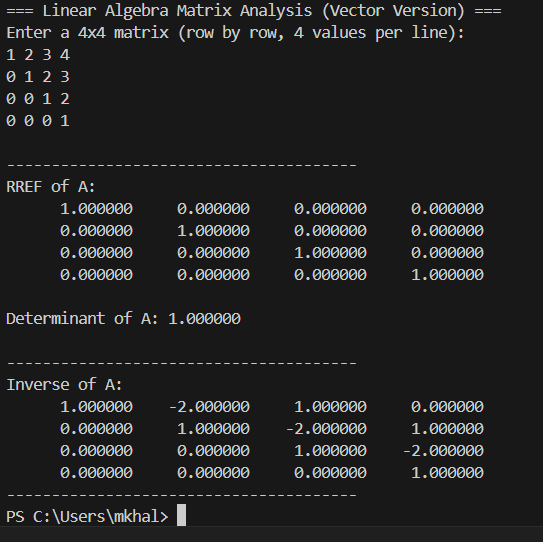
\includegraphics[width=0.5\linewidth]{f1.png}
    \caption{Program output for the invertible matrix M.}
    \label{fig:output_m}
\end{figure}

\subsubsection{Example 2: Non-Invertible Matrix N}
Consider the non-invertible matrix $N$, where the third row is a linear combination of the first two ($R_3 = R_1 + R_2$):
\[
N = 
\begin{bmatrix}
1 & 2 & 3 & 4 \\
5 & 6 & 7 & 8 \\
6 & 8 & 10 & 12 \\
9 & 10 & 11 & 12
\end{bmatrix}
\]
The program's output, shown in Figure 2, confirms that $N$ is singular. The RREF contains a zero row, the determinant is zero, and the program reports that the matrix is not invertible.

\begin{figure}[h!]
    \centering
    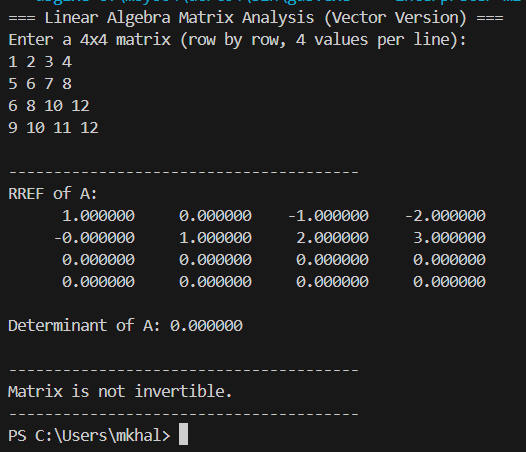
\includegraphics[width=0.5\linewidth]{f2.png}
    \caption{Program output for the non-invertible matrix N.}
    \label{fig:enter-label}
\end{figure}


\section{Adjoint of a matrix}
\defn{The Adjoint of a Matrix}{Adjoint}
{Let $A$ be any square matrix. The cofactor matrix of $A$, denoted by $cof(A)$, is the matrix whose
$(i, j)-$entry is the $(i, j)-$cofactor $C_{ij}$ of the matrix $A$. The adjoint of $A$, denoted by $adj(A)$, is defined to
be the transpose of its cofactor matrix.
\[adj(A) = (cof(A))^T\]
The adjoint is also known as adjugate or adjunct. In this section, you need to do the following.}
\thmp{}{}
{
For any $n \times n$ matrix $A$ we have that: \[A\ adj(A)= det(A)\ I_n\]
}
{
Let $A=[a_{ij}]$ be an $n \times n$ square matrix. By definition of matrix multiplication, we define $A\ adj(A)=S$, but we know that the adjoint of $A$ is the transpose of the cofactor matrix of $A$ and we define it by $D=[d_{ij}]$. \[\text{Thus, }[s_{ij}]=\sum_{k=1}^na_{ik} \ d_{kj}=\sum_{k=1}^na_{ik} \ C_{jk}.\]
We notice that we have two cases for the values of $i,j$:\\

\textbf{Case 1} $(i=j)$: This case is for the main diagonal entries of the product matrix. Then we get \[[s_{ii}]=\sum_{k=1}^na_{ik} \ C_{ik}\]
By definition of matrix multiplication and cofactor expansion, we see that $s_{ii} =\sum_{k=1}^na_{ik} \ C_{ik}= det(A)$, in other words, every main diagonal entry of the adjoint matrix of $A$ is the determinant of $A$.\\

\textbf{Case 2} $(i\neq j)$: This case is for the off-diagonal entries.\[[s_{ij}]=\sum_{k=1}^na_{ik} \ C_{jk}\]
We construct a matrix $B$ by copying the matrix $A$ and replacing the $j^{th}$ row of $B$ by a copy from the $i^{th}$ row of $A$. So, the $i^{th}$ and $j^{th}$ rows of $B$ are identical. Thus, $s_{ij}=\sum_{k=1}^na_{ik} \ C_{jk}=\sum_{k=1}^na_{jk} \ C_{jk}=det(B).$ But we know that $B$ has two identical rows, so its determinant is zero. Hence, $s_{ij}=0$, where $i \neq j.$
\\
Therefore, \[A \ adj(A)= \begin{bmatrix}
    det(A)&0&0&\dots&0\\
    0&det(A)&0&\dots&0\\
    0&0&det(A)&\dots&0\\
    \vdots&\vdots&\vdots&\ddots&\vdots\\
    0&0&0&\dots&det(A)
\end{bmatrix} = det(A) \begin{bmatrix}
    1&0&0&\dots&0\\
    0&1&0&\dots&0\\
    0&0&1&\dots&0\\
    \vdots&\vdots&\vdots&\ddots&\vdots\\
    0&0&0&\dots&1
\end{bmatrix}=det(A)I_n, \]
which satisfies the proof.
} \newpage
\section{Verification of the Theorem}

We now verify the theorem
\[
A\,\operatorname{adj}(A) = \det(A)\,I_n
\]
for two concrete examples: an invertible matrix $M$ and a singular (non-invertible) matrix $N$.

\subsection*{Example 1: Invertible matrix $M$}

Consider the invertible matrix
\[
M =
\begin{bmatrix}
1 & 2 & 3 & 4 \\
0 & 1 & 2 & 3 \\
0 & 0 & 1 & 2 \\
0 & 0 & 0 & 1
\end{bmatrix}.
\]

\paragraph{Step 1: Determinant of $M$.}
Since $M$ is upper triangular, the determinant is the product of the diagonal entries:
\[
\det(M) = 1 \times 1 \times 1 \times 1 = 1.
\]

\paragraph{Step 2: Cofactor and Adjoint of $M$.}
The cofactor matrix $cof(M)$ is computed as:
\[
cof(M) =
\begin{bmatrix}
1 & 0 & 0 & 0\\
-2 & 1 & 0 & 0\\
1 & -2 & 1 & 0\\
0 & 1 & -2 & 1
\end{bmatrix}.
\]

Taking its transpose gives the adjoint:
\[
\operatorname{adj}(M) = cof(M)^T =
\begin{bmatrix}
1 & -2 & 1 & 0\\
0 & 1 & -2 & 1\\
0 & 0 & 1 & -2\\
0 & 0 & 0 & 1
\end{bmatrix}.
\]

\paragraph{Step 3: Verifying the theorem.}
Now multiply:
\[
M\,\operatorname{adj}(M)=
\begin{bmatrix}
1 & 2 & 3 & 4 \\
0 & 1 & 2 & 3 \\
0 & 0 & 1 & 2 \\
0 & 0 & 0 & 1
\end{bmatrix}
\begin{bmatrix}
1 & -2 & 1 & 0\\
0 & 1 & -2 & 1\\
0 & 0 & 1 & -2\\
0 & 0 & 0 & 1
\end{bmatrix}
=
\begin{bmatrix}
1 & 0 & 0 & 0 \\
0 & 1 & 0 & 0 \\
0 & 0 & 1 & 0 \\
0 & 0 & 0 & 1
\end{bmatrix}
= \det(M)\,I_4.
\]

Thus the theorem holds for $M$.

\bigskip
\subsection*{Example 2: Singular matrix $N$}

Consider the singular matrix
\[
N =
\begin{bmatrix}
1 & 2 & 3 & 4 \\
5 & 6 & 7 & 8 \\
6 & 8 & 10 & 12 \\
9 & 10 & 11 & 12
\end{bmatrix}.
\]

Notice that the third row is a linear combination of the first two ($R_3 = R_1 + R_2$), so the rows are linearly dependent. Hence:
\[
\det(N) = 0.
\]

By the theorem:
\[
N\,\operatorname{adj}(N) = \det(N)\,I_4 = 0_{4\times4}.
\]

This confirms the result for a singular matrix.

\bigskip
\subsection*{Formula for the Inverse using the Adjoint}

If $A$ is invertible (i.e., $\det(A)\neq 0$), the theorem gives:
\[
A\,\operatorname{adj}(A) = \det(A)\,I_n.
\]
Multiplying both sides by $\dfrac{1}{\det(A)}$:
\[
A \left( \frac{\operatorname{adj}(A)}{\det(A)} \right) = I_n.
\]
Thus,
\[
\boxed{A^{-1} = \frac{\operatorname{adj}(A)}{\det(A)}.}
\]

\subsection*{Example: Computing $M^{-1}$}

For the invertible matrix $M$, we have $\det(M)=1$ and:
\[
cof(M) =
\begin{bmatrix}
1 & 0 & 0 & 0 \\
-2 & 1 & 0 & 0 \\
1 & -2 & 1 & 0 \\
0 & 1 & -2 & 1
\end{bmatrix},\quad
\operatorname{adj}(M) = cof(M)^T =
\begin{bmatrix}
1 & -2 & 1 & 0 \\
0 & 1 & -2 & 1 \\
0 & 0 & 1 & -2 \\
0 & 0 & 0 & 1
\end{bmatrix}.
\]

Therefore:
\[
M^{-1} = \frac{\operatorname{adj}(M)}{\det(M)} = \operatorname{adj}(M).
\]

This matches the inverse computed by our algorithm (see Figure~\ref{fig:output_m}).

\end{document}

